%!TEX root = practicum2.tex
\begin{figure*}
	\centering
	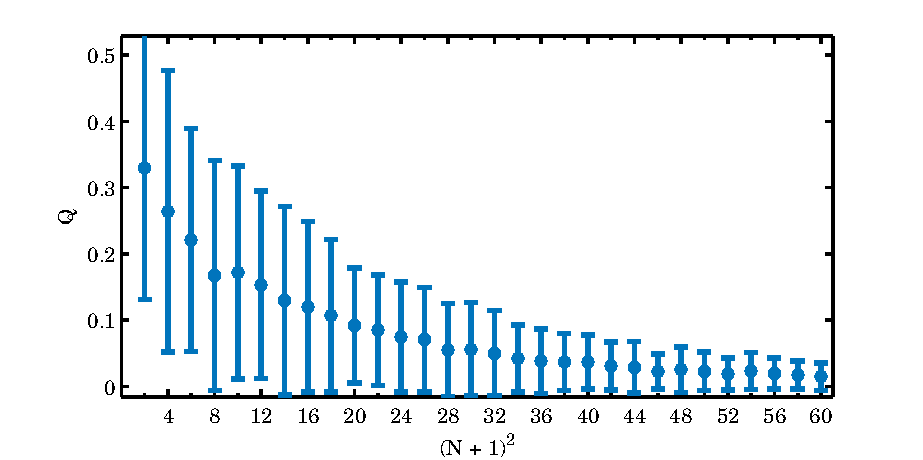
\includegraphics[width=\textwidth]{./img/assignment_b_mean_std_n.pdf}
	\caption{The mean, represented as points, and standard deviations, indicated by the error bars, of the ratio of the cluster size to number of sites in the grid, i.e. $(N + 1)^2$.The mean and standard deviation were calculated over $200$ runs with $p = 0.5$.}
	\label{fig:experiment:size:mean_std_clusters}
\end{figure*}

In \cref{ss:exp:probability} we postulated that our relatively small grid influenced the found value of $p_c$. This section qualitatively discusses the relation between the size of the grid and the cluster. We repeat the experiment discussed in \cref{ss:exp:probability} but varied $N = 2, 6, \dotsc, 60$ instead of $p$. Since we are mostly interested in the size of finite clusters we choose $p = 0.5 < p_c$. Instead of the size of grid we now measure $Q$ the ratio of the size of finite clusters to the number of sites in the grid. 

\Cref{fig:experiment:size:mean_std_clusters} shows the mean and standard deviation of $Q$ as a function of $N$. In this graph we observe that the average of $Q$ decreases as $N$ increases, i.e. the size of the clusters does not grow as hard as the number of sites in the grid. \todo{Physics by computer heeft een hoop theorie hiervoer die ik niet helemaal begrijp... of waarvoor we in ieder geval een ander soort plotjes moeten maken.} 

\Cref{fig:experiment:size:prob:p_inf_ratio} shows that $P_\infty$ reaches zero for $N > 40$, which indicates that for this value of $N$ there are no more percolating clusters. This fits with the theory discussed in \cref{ss:exp:probability}, which states that we get only finite clusters for $p < p_c$. We have percolating clusters for $p = 0.5 < p_c$ since the grid is not large enough to hold the finite clusters.\\ 

\begin{figure}
	\centering
	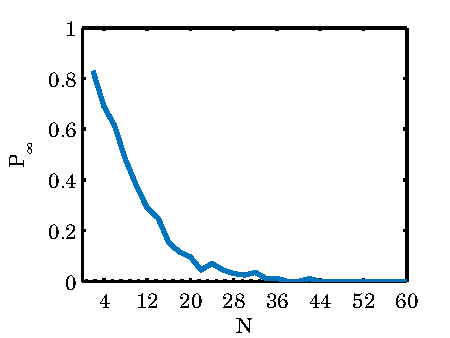
\includegraphics[width=\columnwidth]{./img/assignment_b_p_infinite_ratio_p.pdf}
	\caption{Ratio of percolating clusters to the number of finite clusters, $P_\infty$, as a function of $N$. Ratios are calculated over $r_{max} = 200$ runs with $p = 0.5$.}
	\label{fig:experiment:size:prob:p_inf_ratio}
\end{figure}

% Behaviour in the limit. 
If the lattice size is infinite we are no longer limited by the size of the lattice, in essence we remove one of our stop conditions. In this situation the theory presented in \cref{ss:exp:probability} holds, i.e. as long as $p < p_c$ we only have finite clusters. As $p > p_c$ the number of percolating clusters relative to the number of finite clusters increases until we always get a percolating cluster for $p = 1$.

	